\subsubsection{Login}
Wie in Abbildung \ref{fig:login_reliability_score} zu sehen ist, hat jeder Testdurchlauf beim Average Load Test vom Login ein Scoring von über 60 von 100 Punkten erreicht.
Dabei konnte die k3s-Umgebung jedes Mal ein höheres Scoring als die Docker-Compose-Umgebung erzielen.

Interessant ist der höhere maximale CPU-Verbrauch der Anwendung in der Docker-Compose-Umgebung im Vergleich zur k3s-Umgebung, wie in Tabelle \ref{tab:login_average_load_metrics} zu sehen ist.
Während der maximale CPU-Verbrauch des gesamten Systems in beiden Umgebungen näher beieinander liegt. Dabei erreicht die Node-CPU-Max aber eine Auslastung von über 100 \%.
\begin{table}[htbp]
\centering
\caption{Vergleich der Durchschnittswerte aller Test zur bestimmung der Zuverlässigkeit für das Login-Szenario unter Average Load}
\label{tab:login_average_load_metrics}

\begin{tabular}{lrr}
\toprule
\textbf{Metrik} & \textbf{Docker} & \textbf{K3s} \\
\midrule
Error Rate [\%]        & 0.0000 & 0.0008 \\
CPU Max [\%]           & 99.45  & 33.47 \\
Memory Max [\%]        & 46.07  & 12.56 \\
Node CPU Max [\%]      & 99.98  & 104.96 \\
Node Memory Max [\%]   & 51.00  & 70.79 \\
Restarts               & 0.00   & 0.00 \\
\bottomrule
\end{tabular}

\end{table}

\begin{figure}[htbp]
\centering
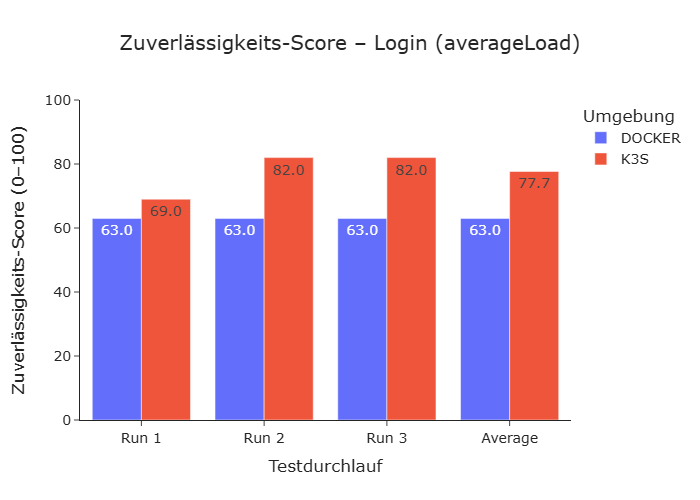
\includegraphics[width=0.8\textwidth]{bilder/tests/reliability_score_login_averageLoad.png}
\caption{Reliability Score für das Login-Szenario unter Average Load}
\label{fig:login_reliability_score}
\end{figure}

Vergleichen wir nun die durchschnittliche Zuverlässigkeit der Score-Werte jedes Tests des Login-Szenarios, die in der Tabelle \ref{tab:scenario_score_matrix_login} zu sehen ist, so zeigt sich, dass die k3s-Umgebung bei jedem Test die bessere Zuverlässigkeit erreicht, bis auf den Smoke-Test bei dem beide die Maximalpunktzahl erreichen konnten.
Bis auf den Spike-Test bleiben beide Umgebungen nah beieinander.

\begin{table}[htbp]
\centering
\caption{Durchschnittlicher Reliability Score pro Testtyp für das Szenario Login}
\label{tab:scenario_score_matrix_login}

\begin{tabular}{lccccc}
\toprule
\textbf{Environment} & \textbf{Smoke} & \textbf{Average Load} & \textbf{Stress} & \textbf{Spike} & \textbf{Breaking Point} \\
\midrule
Docker & 100.00 & 63.00 & 59.67 & 38.00 & 53.00 \\
K3s    & 100.00 & 77.67 & 65.00 & 60.00 & 65.00 \\
\bottomrule
\end{tabular}

\end{table}

\FloatBarrier